% Task 2: collisions of a short digest. The answer (which notes collide) is not shown.
\documentclass[12pt,tikz,border=6pt]{standalone}
% Shared preamble of the task figures of Lecture 7. The colours are the colour roles of the slides
% (main.tex) and of the passwords simulator:
%   Alice sIndigo, Mallory sPink, message / document / password sViolet, salt sAmber,
%   Bob / the server / the notary sTeal, digest sBrown; mechanisms dark; the unknown: orange dashed.
\usepackage{lmodern}
\usepackage[T1]{fontenc}
\renewcommand{\familydefault}{\sfdefault}
\usepackage{amsmath,amssymb}
\usepackage{xcolor}
\usepackage{fontawesome5}
\usetikzlibrary{arrows.meta, calc, positioning, fit, decorations.pathreplacing, backgrounds}

\definecolor{DeepBlue}{HTML}{283593}
\definecolor{AccentOrange}{HTML}{EB5A14}
\definecolor{nInk}{HTML}{37474F}
\definecolor{nLine}{HTML}{90A4AE}
\definecolor{nLight}{HTML}{CFD8DC}
\definecolor{nFill}{HTML}{ECEFF1}
\definecolor{aExec}{HTML}{43A047}
\definecolor{aWrite}{HTML}{E53935}
\definecolor{sIndigo}{HTML}{5C6BC0}
\definecolor{sPink}{HTML}{EC407A}
\definecolor{sViolet}{HTML}{7E57C2}
\definecolor{sAmber}{HTML}{FFB300}
\definecolor{sTeal}{HTML}{26A69A}
\definecolor{sBrown}{HTML}{8D6E63}
\definecolor{sPinkText}{HTML}{C2185B}
\definecolor{sAmberText}{HTML}{A06A00}
\definecolor{sTealText}{HTML}{00796B}

\tikzset{
  hw/.style={draw=nLine, thick, fill=nFill, text=nInk, rounded corners=3pt, align=center, inner sep=4pt},
  mech/.style={draw=nInk, thick, fill=nInk, text=white, rounded corners=3pt, align=center, inner sep=5pt, font=\small\bfseries},
  msgval/.style={draw=sViolet, thick, fill=sViolet!12, text=nInk, rounded corners=3pt, align=center, inner sep=4pt},
  saltval/.style={draw=sAmber, thick, fill=sAmber!25, text=nInk, rounded corners=3pt, align=center, inner sep=4pt},
  digval/.style={draw=sBrown, thick, fill=sBrown!15, text=nInk, rounded corners=3pt, align=center, inner sep=4pt},
  srvval/.style={draw=sTeal, thick, fill=sTeal!15, text=nInk, rounded corners=3pt, align=center, inner sep=4pt},
  unk/.style={draw=AccentOrange, thick, dashed, fill=white, text=AccentOrange, rounded corners=3pt, align=center,
    inner sep=4pt, font=\bfseries},
  data/.style={-{Stealth}, very thick, nInk},
  person/.style={circle, fill=#1, draw=#1, text=white, minimum size=1.1cm, font=\Large, inner sep=0pt},
}
\newcommand{\personnode}[4]{%
  \node[person=#3] (#1) at (#2) {\faUser};
  \node[font=\small\bfseries, text=#3, below=0.06cm of #1] (#1lbl) {#4};}
\newcommand{\mallorynode}[2]{%
  \node[person=sPink] (#1) at (#2) {\faUserSecret};
  \node[font=\small\bfseries, text=sPinkText, below=0.06cm of #1] (#1lbl) {Mallory};}
\newcommand{\hashbox}[4]{\node[mech, minimum width=#4] (#1) at (#2) {\faCogs\ #3};}

\begin{document}
\pagecolor{white}
\begin{tikzpicture}[>=Stealth]
  \node[font=\normalsize\bfseries, text=nInk, anchor=west] at (-0.6,2.1) {Hash ``note 0'', ``note 1'', ``note 2'', \ldots\ and keep only the first bits of SHA-256. When does a short digest repeat?};
  \foreach \m/\y in {note 0/1.0, note 1/0.2, note 2/-0.6} {
    \node[msgval, font=\small\ttfamily, minimum width=2.0cm] (m) at (0.5,\y) {\m};
    \node[mech, minimum width=2.6cm, font=\scriptsize\bfseries] (h) at (3.6,\y) {SHA-256, first bits};
    \draw[data] (m) -- (h);
    \node[digval, font=\small\ttfamily, minimum width=1.8cm] (d) at (6.7,\y) {? ? ?};
    \draw[data] (h) -- (d);
  }
  \node[font=\large, text=nInk] at (0.5,-1.3) {\vdots};
  \node[msgval, font=\small\ttfamily, minimum width=2.0cm] (mj) at (0.5,-2.1) {note $j$};
  \node[mech, minimum width=2.6cm, font=\scriptsize\bfseries] (hj) at (3.6,-2.1) {SHA-256, first bits};
  \draw[data] (mj) -- (hj);
  \node[digval, font=\small\ttfamily, minimum width=1.8cm, draw=AccentOrange, line width=1.6pt] (dj) at (6.7,-2.1) {seen before!};
  \draw[data] (hj) -- (dj);
  \node[hw, text width=5.4cm, align=left, font=\small, anchor=west] (tb) at (8.4,-0.4) {\faTable\ \textbf{seen}: a table\\ short digest $\rightarrow$ note number\\[3pt] \scriptsize like a hash table in C};
  \draw[data, dashed] (6.7,-0.95) -- (tb.west);
  \node[font=\small, text=nInk, anchor=west, align=left] at (-0.6,-3.2) {Sizes: \textbf{24}, \textbf{32}, \textbf{40} bits. Prediction: about $1.18 \cdot 2^{n/2}$ notes. Your answer: $i$ = ?, $j$ = ?};
\end{tikzpicture}
\end{document}
